\section{Busca Binária}

\begin{frame}[fragile]\frametitle{Busca binária}

	\begin{itemize}
		\item A busca binária se vale da ordenação de um vetor de $N$ elementos para acelerar o 
        processo de busca

		\item A ordem de complexidade da busca binária é $O(\log N)$

		\item O vetor deve estar em ordem crescente

        \item A busca binária identifica, primeiramente, o elemento $m$ que está na posição central         do intervalo $[a, b]$ ($m = (a + b)/2$) e o elemento $x$ a ser localizado

        \item Se $x = m$, a busca retorna verdadeiro; caso contrário, ela compara os valores de $x$         e $m$

        \item Se $x < m$, a busca reinicia no intervalo à esquerda de $m$ ($[a, m - 1]$); 
        se $x > m$, a busca continua no subvetor à direita da $m$ ($[m + 1, b]$)

        \item Se $b < a$, a busca returna falso
	\end{itemize}
 
\end{frame}  

\begin{frame}[fragile]{Visualização da busca binária}

    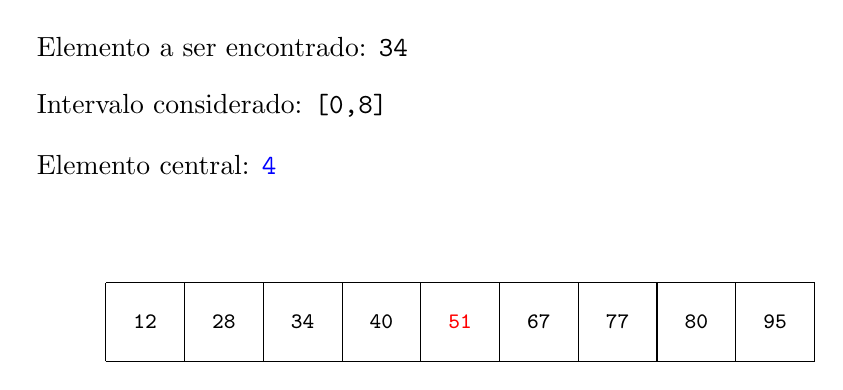
\begin{tikzpicture}
        \node[anchor=west] at (0, 4) {Elemento a ser encontrado: \texttt{34}};
        \node[anchor=west] at (0, 3.25) {Intervalo considerado: \texttt{[0,8]}};
        \node[anchor=west] at (0, 2.5) {Elemento central: \texttt{\textcolor{blue}{4}}};
        \draw (1,0) grid (10,1);

        \node at (1.5,0.5) {\footnotesize \texttt{12}};
        \node at (2.5,0.5) {\footnotesize \texttt{28}};
        \node at (3.5,0.5) {\footnotesize \texttt{34}};
        \node at (4.5,0.5) {\footnotesize \texttt{40}};
        \node at (5.5,0.5) {\footnotesize \texttt{\textcolor{red}{51}}};
        \node at (6.5,0.5) {\footnotesize \texttt{67}};
        \node at (7.5,0.5) {\footnotesize \texttt{77}};
        \node at (8.5,0.5) {\footnotesize \texttt{80}};
        \node at (9.5,0.5) {\footnotesize \texttt{95}};
    \end{tikzpicture}

\end{frame}

\begin{frame}[fragile]{Visualização da busca binária}

    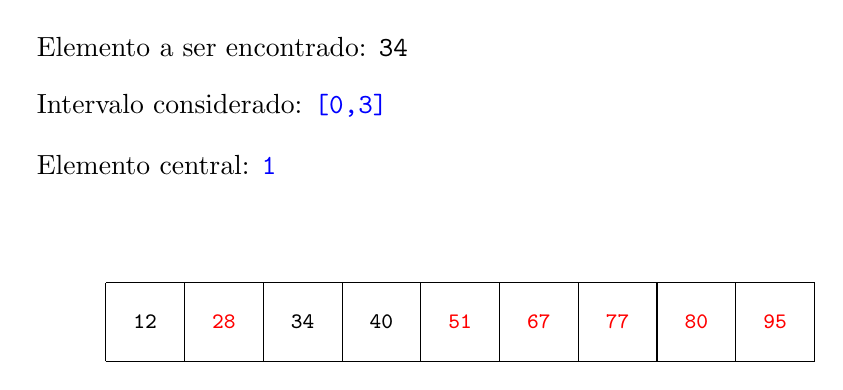
\begin{tikzpicture}
        \node[anchor=west] at (0, 4) {Elemento a ser encontrado: \texttt{34}};
        \node[anchor=west] at (0, 3.25) {Intervalo considerado: \texttt{\textcolor{blue}{[0,3]}}};
        \node[anchor=west] at (0, 2.5) {Elemento central: \texttt{\textcolor{blue}{1}}};
        \draw (1,0) grid (10,1);

        \node at (1.5,0.5) {\footnotesize \texttt{12}};
        \node at (2.5,0.5) {\footnotesize \texttt{\textcolor{red}{28}}};
        \node at (3.5,0.5) {\footnotesize \texttt{\textcolor{black}{34}}};
        \node at (4.5,0.5) {\footnotesize \texttt{40}};
        \node at (5.5,0.5) {\footnotesize \texttt{\textcolor{red}{51}}};
        \node at (6.5,0.5) {\footnotesize \texttt{\textcolor{red}{67}}};
        \node at (7.5,0.5) {\footnotesize \texttt{\textcolor{red}{77}}};
        \node at (8.5,0.5) {\footnotesize \texttt{\textcolor{red}{80}}};
        \node at (9.5,0.5) {\footnotesize \texttt{\textcolor{red}{95}}};
    \end{tikzpicture}

\end{frame}

\begin{frame}[fragile]{Visualização da busca binária}

    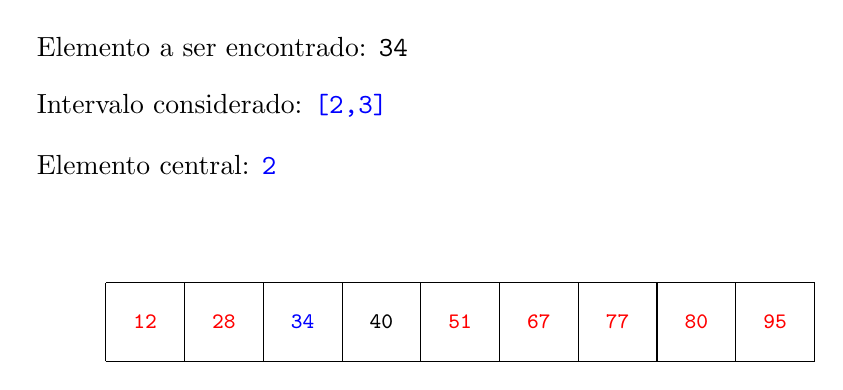
\begin{tikzpicture}
        \node[anchor=west] at (0, 4) {Elemento a ser encontrado: \texttt{34}};
        \node[anchor=west] at (0, 3.25) {Intervalo considerado: \texttt{\textcolor{blue}{[2,3]}}};
        \node[anchor=west] at (0, 2.5) {Elemento central: \texttt{\textcolor{blue}{2}}};
        \draw (1,0) grid (10,1);

        \node at (1.5,0.5) {\footnotesize \texttt{\textcolor{red}{12}}};
        \node at (2.5,0.5) {\footnotesize \texttt{\textcolor{red}{28}}};
        \node at (3.5,0.5) {\footnotesize \texttt{\textcolor{blue}{34}}};
        \node at (4.5,0.5) {\footnotesize \texttt{\textcolor{black}{40}}};
        \node at (5.5,0.5) {\footnotesize \texttt{\textcolor{red}{51}}};
        \node at (6.5,0.5) {\footnotesize \texttt{\textcolor{red}{67}}};
        \node at (7.5,0.5) {\footnotesize \texttt{\textcolor{red}{77}}};
        \node at (8.5,0.5) {\footnotesize \texttt{\textcolor{red}{80}}};
        \node at (9.5,0.5) {\footnotesize \texttt{\textcolor{red}{95}}};
    \end{tikzpicture}

\end{frame}

\begin{frame}[fragile]{Exemplo de uso de busca binária}
    \inputsnippet{c}{13}{29}{quadrinhos2.c}
\end{frame}

\begin{frame}[fragile]{Busca binária em C/C++}

    \begin{itemize}
		\item A função \code{c}{bsearch()} da biblioteca \code{c}{stdlib.h} do C implementa a busca 
        binária

        \item A sintaxe da função \code{c}{bsearch()} é
            \inputsyntax{c}{bs.st}

        \item A biblioteca \code{c++}{algorithm} do C++ traz três funções associadas à busca
            binária

        \item A função \code{c++}{binary_search()} retorna verdadeiro se o elemento a ser
        encontrado está no intervalo indicado
            \inputsyntax{c++}{binary_search.st}

        \item As funções \code{c++}{lower_bound()} e \code{c++}{upper_bound()} retorna um iterador
        para o primeiro elemento maior ou igual a $x$, ou estritamente maior do que $x$, 
        respectivamente:
            \inputsyntax{c++}{bounds.st}
    \end{itemize}

\end{frame}

\begin{frame}[fragile]{Exemplo de uso de busca binária em C e C++}
    \inputsnippet{c++}{1}{21}{cbs.cpp}
\end{frame}

\begin{frame}[fragile]{Exemplo de uso de busca binária em C e C++}
    \inputsnippet{c++}{23}{43}{cbs.cpp}
\end{frame}
